\documentclass[11pt]{article}
\usepackage[a4paper, top=4cm, bottom=3cm, left=3cm, right=3cm]{geometry}
\usepackage{geometry} % see geometry.pdf on how to lay out the page. There's lots.
\geometry{a4paper} % or letter or a5paper or ... etc
% \geometry{landscape} % rotated page geometry
\usepackage[english]{babel}
%\usepackage[utf8]{inputenc}
%\usepackage{accents}
\usepackage{graphicx}
\usepackage{array}
\usepackage{multirow}
%\usepackage{mathptmx}
%\usepackage{amsmath}
%\usepackage{makeidx}
\usepackage{verbatim}
\usepackage{amssymb}
\usepackage{latexsym}
\usepackage{comment}
\usepackage{sectsty}
\usepackage{accents}
\usepackage{natbib}
\usepackage{caption}
% See the ``Article customise'' template for come common customisations
\newcolumntype{x}[1]{{\centering\hspace{0pt}}p{#1}}

% By Simon ==================================================


\newcommand{\simon}[1]{\vspace{1em}(\emph{Simon: #1})\vspace{1em}}

%TIKZ====
\usepackage{tikz}
\usetikzlibrary{arrows,shadows,petri,positioning}
%\usetikzlibrary{fit}					% fitting shapes to coordinates

% End by Simon =============================================


\title{ICT for Basic Service Delivery - Case Study: Water Sector in Uganda}
\author{
\small{Ikae Catherine Omal}\\
\small{School of Computing and Informatics Technology, University of Makerere, Uganda}\\ \small{\textit{ikae.catherine@cit.mak.ac.ug}}\\
}

\date{\today}

\begin{document}
\maketitle

\begin{abstract}
To be completed
\end{abstract}



%%%%%%%%%%%%%%%%%%%%%%%%%%%%%%%%%%%
%Introduction
\section{Main objectives and research hypotheses}\label{objectives}
The main objective will be to understand how mobile phone services can be improved and adjusted to the combined context of developing countries (Uganda) and crowdsourced monitoring (water maps) to ensure improved access to water. Our main assumption is that up-to-date and accurate information is crucial for the correct allocation of resources and budget dedicated to water infrastructures. This is the also the assumption shared by many new water mapping projects in Africa\footnote{Rural Water Supply Network (RWSN): http://www.rural-water-supply.net/en/}. Such a research is therefore especially crucial at a time when more and more institutions (governments and NGOs) are relying on end-user provisions of infrastructure information to allocate new investments and to ensure general quality of services. For example, new ``crowd-­maps"\footnote{Crowd maps allow anybody to provide geo-­based information (e.g. reports, reviews, or pictures) on topics that are important for them and for front providers and governments.} have been set up to capture the status of important infrastructure (Ushahidi, NextDrop, H20initiative), requested actions for failing infrastructure (Huduma) or crucial news in times of conflicts or disasters (Libya Crisis Map, Geofeedia), with varying degrees of success. 
\\
In the typical African context of largely scattered rural populations, the ability to use sms-based monitoring on services access can greatly reduce monitoring costs and misallocations, a priority for budget-constrained governments. It promises also better governance through greater transparency and increased participation from end-users. According to the World Bank (2004), ``successful services for poor people emerge from institutional relationships in which the actors are accountable to each other". Shared information and communication could therefore be an attractive solution to foster these mutual accountabilities. 
\\\\
However, while the benefits of mobile-based, user-centric information seem clear, the level of participation accross communities remain very low, both in terms of external intensity (the number of people using the mobile reporting tools) and internal intensity (the number of messages sent back to the central entity). Without the full participation of end-users, most ICT projects are destined to fail, which represents a massive opportunity loss. Our assumption is that most of this problem is due to an  inadequation between the mobile services and their targeted demographic, in terms of ease of use (language, interface), incentives (absence of feedbacks and recompense for the effort) and social dynamics (target the individuals in a community-driven context). When a system is simple to use and has clear value (such as m-payment MPESA), uptake and usage rates are much higher. We aim to attain a same level of participation for the provision of information destined to populate water maps.  
\\\\
To succesfully achieve this goal, the proposed research will form a sequence of 4 different research ``modules":
\begin{enumerate}
\item
We will analyze the current context in our target research field: who are the people using phones; what are the current ICT (mostly phones) penetration, usages and types (simple or smartphone); what are the biggest barriers to usage (complexity, lack of perceived rewards, technical hurdles); what are the forms and frequency of mobile communications (sms, voice...); what is the recognized value of monitoring and reporting on water infrastructure.
\item
We will experiment with the designs of the communication channels/ user-interfaces (UI) used to provide the bottom-up information on water: nature of the message (sms, mail, voice…), language used (multi-lingual, symbol-based), actions required (forms, dialed-in choice selection, special number-to-action, voice messengers…). In general, choices about design will be informed by the results of the context analysis. Each interface will then be tested in a randomized experiment to assess its effectiveness on the amount of data sent back (data density) and to account for the influence of external drivers (education, gender, wealth...)
\item
Following the experimental pattern of the previous module, we further experiment with the implementation of feedbacks and rewards messages to inform the end-users about the value of water reporting. 
This aspect is especially important since we expect the lack of feedbacks to be one of the key drivers of low participation levels accross many water mapping projects.
We also plan to integrate network-centric rewards such as community checks (e.g. cross-validation of messages) or possible gamification tools (e.g. points-to-purchase scheme) to improve internal intensity. 
\item
Finally and using the collected information, we will test for the nature of the data sent back (data quality), in terms of content and degree of details. Modules of pattern recognition (via machine-learning) will be implemented to categorize and classify data and to assess the influence communication channels and feedback schemes have on the quality of information collected (while accounting for socio-economic characteristics). This aspect should give us insights generalizable to other sectors and functions.
\item
\end{enumerate}  
\\\\
The thesis will be part of a larger multi-disciplinary project on "mobile ICT for public services under weak public institutions" under the joint supervision of Ass. Prof. Isabel Günther (ETH NADEL), Prof. Gerhard Tröster (ETH Electronic Labs) and Prof. Helbing (ETH SOMS) and with the active colaboration of several research insitutes in Switzerland and in sub-Saharan Africa (ETH-­NADEL, ETH-­SOMS, ETH-­Electronics Lab for Switzerland, Makerere School of Computing and IT for Uganda, iHub Research for Kenya, and University of Dar es Salaam for Tanzania). In particular, the field part of the thesis will be coordinated with Prof. Florence Tushabe at the School of Computing and IT at Makerere University (Uganda). The water-related aspects will benefit from close interactions with Dr. Richard Johnston from EAWAG (Zurich) and from Dr. Niwagaba from the Civil and Environmental Engineering Department at Makerere University.  

\section{Field context}
\subsection{Targeted region}
For the implementation of this proposed doctoral thesis, we target the Ugandan district of Wakiso, which has a total area of 2,704 km$^{2}$ and an estimated total population of 1,310,100. It is made up of two counties: Kyaddondo County and Busiro County. 
\\
Considering that the district cannnot be covered in its entirety due to time and budget constraints, the proposed field target is the Kakiri Municipality, which lies approximately 17 kilometres northeast of the central business district of the city of Kampala, the Uganda's capital. This town presents multiple advantages for the success of this project: it is close to the capital, with an important and easily accessible population and with a evenly distributed gender population (48.5\% of men for 52.2\% of women, according to \citep{population2010} and \citep{population02}). Across the other key characteristics of interest (wealth, education, type of employment, source of revenues, water access), the municipality spans a large variety of education, activity and wealth profiles. It is also at the junction of urban and rural activities, which will allow for some analysis of the urban/rural potential discrepencies. Moreover and quite importantly, water access is difficult, collective and the frequent object of tension in the population. It is therefore an excellent field for assesssing new ICT devices target water management and provision.
\subsection{Current ICT context}
Based on a rapid field survey in the Kakiri municipality, it appears that most people are embracing mobile phone technologies and using them on a daily basis, not only to access but also to share information freely. In general, mobile phones have become basic needs to many Ugandans because people rely on them to access a wide range of services: from market prices to mobile banking (Mobile Money) to Mobile Health (mHealth).
Moreover, mobile phones are used more and more for data collection and dissemination across multiple sectors, such as health, socio-economic development, agriculture, natural resource management, disaster relief, and their relevant subsectors. In health, or mHealth, mobile phones are employed to (i) disseminate information on public health to residents and health workers, (ii) collect real-time data, (iii) assist in and monitor medication compliance, (iv) track disease outbreaks, (v) manage inventories of drugs in remote locations. In agriculture, mobile phones connect farmers to government services, cooperatives, and networks, as well as facilitate the flow of timely information about markets and crop prices. Mobile banking, or mBanking, has made financial services more attractive and readily accessible to poor populations and those living in remote locations\cite{Rikke10}. Mobile phones hold particular value in these fields because they can act as point-of-use devices, function in remote locations, and are readily carried and used at any time \cite{Kimberly11}\cite{Rikke10}.
\\
However, the ICT penetration and the new services favored in the urban and concentrated areas of Uganda do not really apply to the rural context. Studies have revealed that rural inhabitants and poorer urban users value phone services but do not use them very often compared to relatively more affluent users; over 40\% of people in Uganda used mobile phones through friends and family and individuals; although a further 24\% of people used mobile phone through teleshops, demonstrating a strong preference for mobile phones rather than landline phones, and a preference for private phones rather than public access points. It has also been shown that “chatting” with friends and family is clearly the most common use of phones in Uganda\cite{ Scott04}.

\section{State of research in the field}\label{state_of_research}
Should cover state of research and references (point3), and innovativeness of research/ research methodology (point4) + corresponding logical framework (whatever that is)

\simon{To Do}

\section{Methodology}\label{methodology}
\subsection{Methodology}\label{metho}
Should give in full details the methodology to be used (point4)

\begin{figure}
\begin{center}
 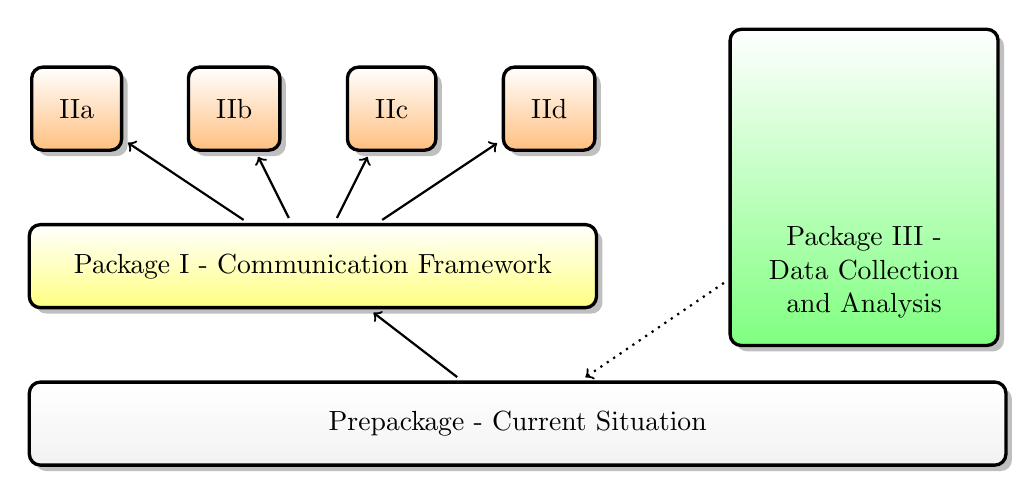
\begin{tikzpicture}[node distance=1.5cm, shorten >=2pt, shorten <=2pt, thick, auto]


\tikzstyle{box} = [
    rectangle,rounded corners,draw=black, top color=white, very thick, inner sep=1em, minimum size=3em,drop shadow]

 
\node[box, bottom color=gray!10, text width = 11.7cm, text centered] at (-1.4,0) (prepackage) {Prepackage - Current Situation};

\node[box, bottom color=yellow!50, text width = 6.5cm, text centered] at (-4,2) (packagei) {Package I - Communication Framework};

\node[box, bottom color=green!50,  text width = 2.7cm, text height = 2.4cm, text centered] at (3,3) (packageiii) {Package III - Data Collection and Analysis};


\node[box,  bottom color=orange!50] at (-7,4) (packageiia) {IIa};

\node[box,  bottom color=orange!50] at (-5,4) (packageiib) {IIb};

\node[box,  bottom color=orange!50] at (-3,4) (packageiic) {IIc};

\node[box,  bottom color=orange!50] at (-1,4) (packageiid) {IId};



\path[->]
  (prepackage) edge (packagei)
  (packagei) edge (packageiia)
  (packagei) edge (packageiib)
  (packagei) edge (packageiic)
  (packagei) edge (packageiid)
;

\path[->, dotted]
  (packageiii) edge (prepackage)
;


\end{tikzpicture} 
\end{center}
\caption{Research packages hirarchy}
\label{tikz:researchpackages}
\end{figure} 

Champanis and Rivett \cite{champanis2012reporting} state: \begin{quote}
``Based on our experience and focus on rural environments, our
approach to ICT development has been that the investigation of
the local context and solutions responding to local needs are more
valuable and sustainable than a general “one-size-fits-all” design.
Whilst this speaks against the notions of “scalability”, which is
usually a desired outcome for IT solutions, we believe that rural
and under-resourced environments require a more detailed and
customised solution.''\end{quote} 

A set of research packages is presented that allows to build up a well tailored but still scalable solution that - beside of helping people directly -  gives space to investigate on research relevant questions in the field of computer science and further sociology, development aid and economics. 

The small Prepackage analyses the context. In Package I the main framework for future project plug-ins is designed. The actual scientific part from a computer science perspective is done in Package II whose subpackages can be implemented individually. Package III is a parallel ongoing process that profits from improvements in Packages I\&II (See Figure~\ref{tikz:researchpackages}).
\subsubsection*{Prepackage: Analysis of the current situation}
\paragraph{Goal} Get an overview of mobile ICT usage and water management in rural Uganda.
\paragraph{Method}
In the field of moile ICT information is aggregate from cooperation with governmental institutions, local service provides and in detailed literature study.
\begin{enumerate}
 \item Distribution of cell phones (by model, user age, area)
 \item Usage distribution (by time, frequency and service)
 \item Analysis of finances (income per user, cost of different services per user, money spent for different services per user)
 \item Analysis of technology (cellular network standards, cell sizes, user per cells, quality of service, future investments, availability of electricity)
 \item Analysis of hindrances for a more frequent usage (finances, easy of use, illiteracy, privacy concerns)
\end{enumerate}
In the field of drinking water we can additional profit from partnership with local NGOs.
\begin{enumerate}
 \item Analysis of the drinking water need amongst population and its challenges
 \item Further data we will be collected during the project as a result of Package III
\end{enumerate}







\subsubsection*{Package I: Design of a communication channel}
\paragraph{Goal} Design a inter-user communication channel that is user friendly, low-cost, reliable, secure and information rich.
\paragraph{Method} A first substep evaluates different communication channels. Text-, graphical- and voice based methods are compared on different generations of phones. Depending on their connection standards (GSM, GPRS, 3G) and application platforms supported (SMS, Java Me, Android) best possible options are chosen. Challenges occur in the following areas:
\begin{itemize}
 \item Low cost feature phones (``a modern low-end mobile phone that is not a smart phone'' [Wikipedia]) are widely available in Uganda. Their drawback is that software has to be implemented manufacturer depending and in general allows just limited functionality \cite{champanis2012reporting}.
 \item Access to provider data (calls with user id, text messages, cell info) is difficult to obtain. A possible solution is to use just mobile data services and transfer messages based on an extra developed service.
 \item Literacy rate of Uganda is around 66 percent [Wikipedia]. Tailored solutions for illiterates have successfully been implemented \cite{brown2012water}. By developing special input methods, one has to be aware that a very important reason for people to buy a phone is due to its associated status and not its features \cite{knoche2012text}.
 \item Low cost transmission is necessary to achieve a high user participation. Prices for SMS make up a higher percentage of the monthly budget than elsewhere. An alternative approach is to provide hardware and airtime to selected user group to perform studies.
 \item Free hardware and airtime is likely to be misused. Champanis and Rivet report that ``Users would fill up the phone with music and video downloads'' \cite{champanis2012reporting} to an extend that it is not usable for the experiment anymore.
 \item User trust and information security is one of Africas biggest challeng, this due to weak privacy laws, user awareness, political instability and old technology. \cite{goodman2010coming}
\end{itemize}

In a second substep we analyse the information flow needed to provide a water quality information and monitoring network. The implementation (third substep) completes Package I. To the moment it remains an open question if a self designed device for data transmission over the mobile network would fulfil this purpose even better than a cell phone based service. 

The success of such an system is unpredictable. Hence we suggest an iterative approach based on try and error method. Lessons learned from other projects are considered and results reported to the community.



\subsubsection*{Package IIa: Quality control}
\paragraph{Goal} Achieve high quality information collected at a centralised agency but also sent to individual receivers 
\paragraph{Method} According to \cite{birnbaum2012automated} supervised and unsupervised machine learning methods are feasible to classify manually generated data in health surveys in Tanzania and Uganda. Widely used machine learning algorithms could be modified in order to not just classify but rather rate user message according to a scale of trust. Additionally the knowledge of the crowd of users could be used to label messages and hence perform supervised learning on initially unlabelled data - similar to a supervised spam filter. Out of this, a general trust giving and learning (human and machine based) distributed network could be generated.

In this we see the following risks:

\begin{itemize}
 \item The reported lack of data quality in surveys in low income countries could also be the result of the normally used top-down approach \cite{birnbaum2012automated}, whereas a bottom-up approach  (where users have a personal interest on the quality of the data) might not even, or at least less face this problem.
 \item The question resides if a machine learning solution for such a difficult task is an actual benefit for a country where human workforce is cheap (and jobs needed) and technology expensive. We would not be surprised if a mixed solution - highlighting suspicious messages machine- and final classification human based - might be the best solution.
\end{itemize}







\subsubsection*{Package IIb: Context analysis}
\paragraph{Goal}
\begin{itemize}
 \item Season and weather
 \item Location (Cellinfo, GPS)
 \item Analysis of communication channel (extend application to other uses)
 
\end{itemize}

\paragraph{Method}

\subsubsection*{Package IIc: User mapping}
\paragraph{Goal}
\paragraph{Method}

\subsubsection*{Package IId: Incentives and gamification}
\paragraph{Goal}
\paragraph{Method}

\subsubsection*{Package III: Data collection and analysis}
\paragraph{Goal}
\paragraph{Method}



\subsection{Chances and risk associated with selected methodology}\label{risk}
Critical assessment of chances and risks (points8)

\section{Organization}\label{organization}
Should describe in details the institutional framework and the partnership, explaining the contribution of all involved partners (point 5). Clear presentation of the supervision and backstopping (point 6).

\section{Expected results}\label{expected}
Expected results and strategy for their implementation (method or product to be developed and its relevance to end users) (point9)

\section{Budget}
Detailed budget for each year of the scholarship, differentiating all funding sources including those of the ETH chair and partner contributions (financial or in-kind) (point10)


\bibliographystyle{plain}
\bibliography{proposal07022013_jg}


\end{document}